%%%=============BT_1=============%%%
\begin{bt}%[9H2B1]
	Cho tam giác $ABC$ vuông tại $A$ có các cạnh góc vuông $AB = 6$ cm, $AC = 8$ cm. Xác định tâm và tính bán kính đường tròn ngoại tiếp tam giác $ABC$.
	\loigiai{
		\begin{center}
		\begin{tikzpicture}[scale=0.8]
			\coordinate (A) at (0,3);
			\coordinate (B) at (4,0);
			\coordinate (C) at (0,0); % Drawing C at origin to make A and B relative. Wait, A is (0,3), C is (0,0) -> AC vertical. B at (4,0) -> BC horizontal. Right angle at C?
            % Problem says Right at A.
            % Let's Re-orient. A at overlap.
            \coordinate (A) at (0,0);
            \coordinate (B) at (6,0);
            \coordinate (C) at (0,8);
            \draw (A) -- (B) -- (C) -- cycle;
            \coordinate (M) at ($(B)!0.5!(C)$); % Midpoint of hypotenuse
            \draw[dashed] (A) -- (M);
            \draw (M) circle (5cm);
            \node[below left] at (A) {$A$};
            \node[below right] at (B) {$B$};
            \node[above left] at (C) {$C$};
            \node[above right] at (M) {$O$};
            \fill (M) circle (2pt);
             % Mark right angle
            \draw (0.3,0) -- (0.3,0.3) -- (0,0.3);
		\end{tikzpicture}
		\end{center}
		Áp dụng định lý Pythagoras trong tam giác vuông $ABC$:
		\[ BC = \sqrt{AB^2 + AC^2} = \sqrt{6^2 + 8^2} = \sqrt{36 + 64} = \sqrt{100} = 10 \text{ (cm)}. \]
		Tâm đường tròn ngoại tiếp tam giác vuông là trung điểm của cạnh huyền.
		\\
		Vậy bán kính đường tròn ngoại tiếp tam giác $ABC$ là:
		\[ R = \dfrac{BC}{2} = \dfrac{10}{2} = 5 \text{ (cm)}. \]
	}
\end{bt}

%%%=============BT_2=============%%%
\begin{bt}%[9H2B1]
	Cho tam giác đều $ABC$ có cạnh bằng $6$ cm. Tính bán kính đường tròn ngoại tiếp tam giác $ABC$.
	\loigiai{
		\begin{center}
		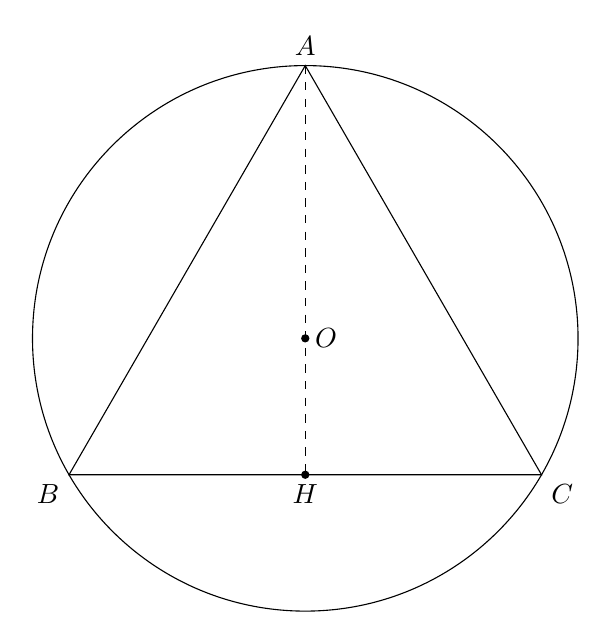
\begin{tikzpicture}[scale=1]
			\coordinate (A) at (0, {6*sqrt(3)/2}); % Height approx 5.2
			\coordinate (B) at (-3,0);
			\coordinate (C) at (3,0);
			\draw (A) -- (B) -- (C) -- cycle;
			\coordinate (O) at (0, {6*sqrt(3)/6}); % Centroid y = h/3 = a*sqrt(3)/6
			\draw (O) circle ({6*sqrt(3)/3}); % R = a*sqrt(3)/3
			\draw[dashed] (A) -- (0,0) node[below]{$H$};
			\node[above] at (A) {$A$};
			\node[below left] at (B) {$B$};
			\node[below right] at (C) {$C$};
			\node[right] at (O) {$O$};
			\fill (O) circle (1.5pt);
            \fill (0,0) circle (1.5pt);
		\end{tikzpicture}
		\end{center}
		Gọi $O$ là tâm đường tròn ngoại tiếp tam giác đều $ABC$, $AH$ là đường cao ($H \in BC$).
		\\
		Đường cao của tam giác đều cạnh $a$ là $AH = \dfrac{a\sqrt{3}}{2} = \dfrac{6\sqrt{3}}{2} = 3\sqrt{3}$ cm.
		\\
		Tâm $O$ cũng là trọng tâm tam giác, nên bán kính $R = OA = \dfrac{2}{3}AH$.
		\[ R = \dfrac{2}{3} \cdot 3\sqrt{3} = 2\sqrt{3} \text{ (cm)}. \]
	}
\end{bt}

%%%=============BT_3=============%%%
\begin{bt}%[9H2B1]
	Cho tam giác $ABC$ cân tại $A$ có $AB = AC = 5$ cm, $BC = 6$ cm. Tính bán kính đường tròn ngoại tiếp tam giác $ABC$.
	\loigiai{
		\begin{center}
		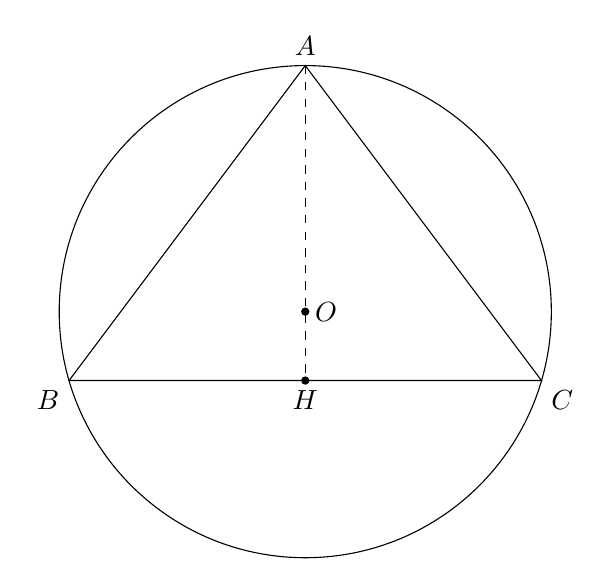
\begin{tikzpicture}[scale=1]
            % BC = 6, so B(-3,0), C(3,0). H(0,0).
            % AB = 5, BH=3 -> AH = sqrt(25-9)=4.
			\coordinate (B) at (-3,0);
			\coordinate (C) at (3,0);
            \coordinate (H) at (0,0);
			\coordinate (A) at (0,4);
			\draw (A) -- (B) -- (C) -- cycle;
            \draw[dashed] (A) -- (H);
            % R = (abc)/(4S) or R = AB^2 / 2h_a
            % R = 25 / (2*4) = 25/8 = 3.125
            \coordinate (O) at (0, {4 - 3.125}); % Center O
            \draw (O) circle (3.125);
			\node[above] at (A) {$A$};
			\node[below left] at (B) {$B$};
			\node[below right] at (C) {$C$};
            \node[below] at (H) {$H$};
			\node[right] at (O) {$O$};
			\fill (O) circle (1.5pt);
            \fill (H) circle (1.5pt);
		\end{tikzpicture}
		\end{center}
		Kẻ đường cao $AH$ ($H \in BC$). Vì $\triangle ABC$ cân tại $A$ nên $H$ là trung điểm $BC \Rightarrow BH = \dfrac{BC}{2} = 3$ cm.
		\\
		Áp dụng định lý Pythagoras trong $\triangle ABH$ vuông tại $H$:
		\[ AH = \sqrt{AB^2 - BH^2} = \sqrt{5^2 - 3^2} = \sqrt{25 - 9} = 4 \text{ (cm)}. \]
		Đặt bán kính đường tròn ngoại tiếp là $R$. Tâm $O$ nằm trên $AH$. Xét $\triangle ABH$:
        Ta có công thức tính nhanh: $R = \dfrac{AB^2}{2AH}$.
		\[ R = \dfrac{5^2}{2 \cdot 4} = \dfrac{25}{8} = 3{,}125 \text{ (cm)}. \]
	}
\end{bt}

%%%=============BT_4=============%%%
\begin{bt}%[9H2B1]
	Cho hình chữ nhật $ABCD$ có $AB = 8$ cm, $BC = 6$ cm. Chứng minh bốn điểm $A, B, C, D$ cùng thuộc một đường tròn và tính bán kính của đường tròn đó.
	\loigiai{
		\begin{center}
		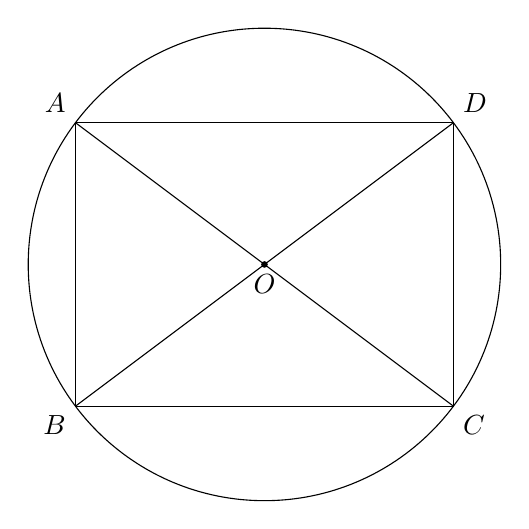
\begin{tikzpicture}[scale=0.6]
			\coordinate (A) at (0,6);
			\coordinate (D) at (8,6);
			\coordinate (C) at (8,0);
			\coordinate (B) at (0,0);
			\draw (A) -- (B) -- (C) -- (D) -- cycle;
            \draw (A) -- (C);
            \draw (B) -- (D);
            \coordinate (O) at (4,3);
            \draw (O) circle (5);
			\node[above left] at (A) {$A$};
			\node[below left] at (B) {$B$};
			\node[below right] at (C) {$C$};
			\node[above right] at (D) {$D$};
			\node[below] at (O) {$O$};
			\fill (O) circle (2pt);
		\end{tikzpicture}
		\end{center}
		Gọi $O$ là giao điểm hai đường chéo $AC$ và $BD$.
		\\
		Theo tính chất hình chữ nhật, ta có $OA = OB = OC = OD$.
		\\
		Vậy bốn điểm $A, B, C, D$ cùng thuộc đường tròn tâm $O$, bán kính $R = OA = \dfrac{AC}{2}$.
		\\
		Xét $\triangle ABC$ vuông tại $B$, theo định lý Pythagoras:
		\[ AC = \sqrt{AB^2 + BC^2} = \sqrt{8^2 + 6^2} = \sqrt{64 + 36} = 10 \text{ (cm)}. \]
		Bán kính đường tròn là:
		\[ R = \dfrac{AC}{2} = 5 \text{ (cm)}. \]
	}
\end{bt}

%%%=============BT_5=============%%%
\begin{bt}%[9H2B1]
	Cho đường tròn $(O; 5 \text{ cm})$. Một dây cung $AB$ có độ dài $8$ cm. Tính khoảng cách từ tâm $O$ đến dây $AB$.
	\loigiai{
		\begin{center}
		\begin{tikzpicture}[scale=0.8]
			\draw (0,0) coordinate (O) circle (2.5); % Scale visual down by half but label as 5
			\coordinate (A) at (-2, 1.5); % Visual coords
            % Need visual calc. R=2.5. AB=4 (scaled). half-chord=2. dist=sqrt(2.5^2 - 2^2)=1.5.
            % So chord at y=-1.5 or +1.5. Let's calculate for 5 and 3.
            % R_vis = 2.5. OH_vis = 1.5. HA_vis = 2.
            \coordinate (O) at (0,0);
            \coordinate (H) at (0,-1.5);
            \coordinate (A) at (-2,-1.5);
            \coordinate (B) at (2,-1.5);
            \draw (O) circle (2.5);
            \draw (A) -- (B);
            \draw[dashed] (O) -- (H);
            \draw[dashed] (O) -- (A);
            \draw (H) rectangle ++(0.2,0.2); % Right angle
			\node[above] at (O) {$O$};
			\node[left] at (A) {$A$};
			\node[right] at (B) {$B$};
            \node[below] at (H) {$H$};
            \node[left, xshift=-2pt, yshift=5pt] at ($(O)!0.5!(A)$) {$R=5$};
			\fill (O) circle (1.5pt);
            \fill (H) circle (1.5pt);
		\end{tikzpicture}
		\end{center}
		Kẻ $OH \perp AB$ tại $H$. Theo quan hệ vuông góc giữa đường kính và dây: $H$ là trung điểm của $AB$.
		\[ HA = HB = \dfrac{AB}{2} = \dfrac{8}{2} = 4 \text{ (cm)}. \]
		Xét $\triangle OHA$ vuông tại $H$:
		\[ OH^2 + HA^2 = OA^2 \]
		\[ OH^2 = OA^2 - HA^2 = 5^2 - 4^2 = 25 - 16 = 9. \]
		\[ \Rightarrow OH = \sqrt{9} = 3 \text{ (cm)}. \]
		Vậy khoảng cách từ tâm $O$ đến dây $AB$ là $3$ cm.
	}
\end{bt}
